\documentclass[letterpaper]{article}
\usepackage[letterpaper]{geometry}
\usepackage{hyperref}
\usepackage{amsmath}
\usepackage{graphicx}
\usepackage{booktabs}

%opening
\title{CS 7641 --- Assignment 3: Unsupervised Learning}
\author{Niranjan Thakurdesai}

\begin{document}
	\maketitle
	
	Three unsupervised learning algorithms, viz. k-means clustering, Gaussian Mixture Models (GMMs) via Expectation Maximization (EM) and Principal Components Analysis (PCA) were analyzed by applying them to the datasets used in assignment 1. The first two are clustering algorithms while the third one is a dimensionality reduction algorithm.
	
	\section{Datasets}
	The same datasets used in assignment 1 were used here. They are provided by UCI Machine Learning and are described briefly below.
	
	\subsection{Dataset 1: Breast Cancer Wisconsin (Diagnostic) Data Set}
	Given features computed from a digitized image of a fine needle aspirate (FNA) of a breast mass, the task is to predict the diagnosis of the tissue (benign or malignant) \cite{streetNuclearFeatureExtraction1993}.
	
	\subsection{Dataset 2: Wine Quality}
	Given physicochemical properties and sensory data of the Portuguese ``Vinho Verde" wine, the task is to predict wine quality \cite{cortezModelingWinePreferences2009}. The dataset related to the white variant of the wine was chosen for experiments since it contains a larger amount of data. The labels in the original dataset are the wine quality measured on a scale from 0 to 10. To facilitate analysis, a cut-off of 6 was chosen. Values above it were relabeled as ‘1’ (good) and those below it as ‘0’ (bad).
	
	\section{Overview of the algorithms}
	The three algorithms and their implementation details are described briefly below.
	
	\subsection{k-means clustering}
	The k-means algorithm clusters data by trying to separate $n$ samples into $k$ clusters by minimizing a criterion called inertia or within-cluster sum of squared distances. After clustering, each sample belongs to the cluster with the nearest mean. The number of clusters $k$ is a user-defined parameter. K-means can be seen as a special case of a GMM with equal covariance per component.
	
	As k-means is extremely sensitive to the initialization of the cluster centers, the `k-means++' initialization method was used \cite{arthurKmeansAdvantagesCareful2007}. This initializes the centroids to be (generally) distant from each other, leading to provably better results than random initialization. Since k-means is not guaranteed to find the global optimum, it was run multiple times with different initializations and the clustering with the lowest inertia was finally chosen.
	
	\subsection{GMMs with EM}
	K-means assumes that each sample is given a ``hard" assignment to exactly one cluster. In contrast to this, GMMs enable soft clustering which gives probabilities of a sample belonging to each cluster. A GMM is a probabilistic model that assumes that all samples are generated from a mixture of a finite number of Gaussian distributions with unknown parameters. This can be thought of as a generalization of k-means to incorporate information about the covariance structure of the data as well as the centers of the latent Gaussians. One advantage of GMM is that it doesn't assume spherical clusters. The number of Gaussians is again a user-defined parameter.
	
	EM is an iterative method to find maximum likelihood of the data by estimating the parameters of the latent Gaussian models. It alternates between performing an expectation (E) step, which creates a function for the expectation of the log-likelihood evaluated using the current estimate of the parameters, and a maximization (M) step, which computes parameters maximizing the expected log-likelihood found on the E step. K-means was used to initialize the Gaussian parameters as it serves as a good initial estimate of the clusters and can speed up convergence.
	
	\subsection{PCA}
	PCA is a dimensionality reduction algorithm used to decompose a multivariate dataset into a set of successive orthogonal components that explain most of the variance in the data. The data can be projected along a subset of these components to reduce its dimensionality.
	
	\section{Experiments and analysis}
	Three kinds experiments were performed:
	\begin{enumerate}
		\item Clustering on the two datasets without dimensionality reduction
		\item Clustering on the two datasets with dimensionality reduction using PCA
		\item Classifying dataset 1 using a neural network after dimensionality reduction
	\end{enumerate}

	K-means uses Euclidean distances while computing inertia. As the features in the datasets are in different scales, features with larger ranges can dominate in the optimization procedure. To prevent this, the datasets are standardized.

	\subsection{Clustering without dimensionality reduction}
	\subsubsection{K-means}
		\begin{figure}
		\centering
		\begin{minipage}{.5\textwidth}
			\centering
			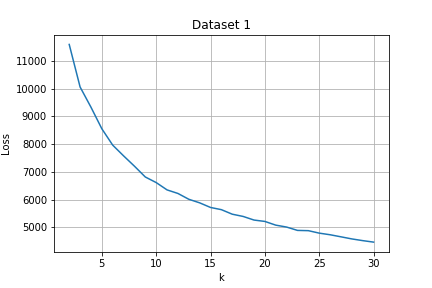
\includegraphics[width=\linewidth]{../../plots/kmeans_loss_1}
			%\caption{Loss curve for RHC}
		\end{minipage}%
		\begin{minipage}{.5\textwidth}
			\centering
			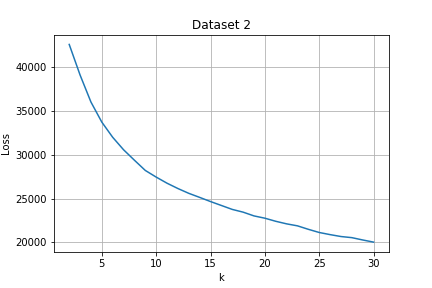
\includegraphics[width=\linewidth]{../../plots/kmeans_loss_2}
			%\caption{Loss for different runs of RHC}		
		\end{minipage}
		\caption{Inertia for different values of k}
		\label{fig:kmeans_losses}%
	\end{figure}%

	Figure \ref{fig:kmeans_losses} shows the inertia for different values of $k$. The elbow method was used to choose the number of clusters. The idea of this method is to choose $k$ by locating the elbow in the loss vs $k$ plot. The elbow is the position where inertia stops decreasing steeply. As observed in the plots, the elbow location isn't clear for both datasets. This may indicate that k-means may not be a good algorithm to find clusters in the data. The approximate elbow location was used, which is $k = 9$ for both datasets.

	Figure \ref{fig:kmeans_hist} shows the distribution of data across clusters. The distribution is quite uneven with some clusters having much more samples than others.
	
	\begin{figure}
		\centering
		\begin{minipage}{.48\textwidth}
			\centering
			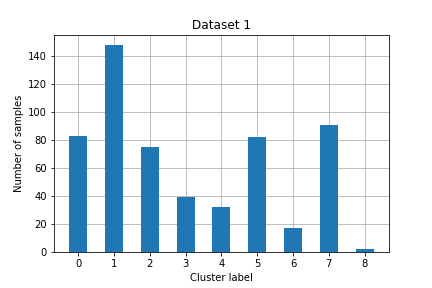
\includegraphics[width=.5\linewidth]{../../plots/kmeans_hist_1}%
			\centering
			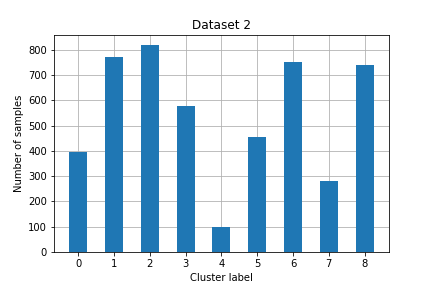
\includegraphics[width=.5\linewidth]{../../plots/kmeans_hist_2}
			\caption{Distribution of samples across k-means clusters (before PCA)}
			\label{fig:kmeans_hist}%
		\end{minipage}%
		\hfill
		\begin{minipage}{.48\textwidth}
			\centering
			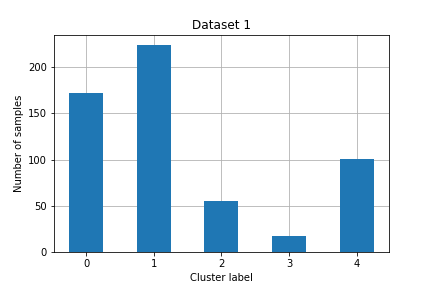
\includegraphics[width=.5\linewidth]{../../plots/gmm_hist_1}%
			\centering
			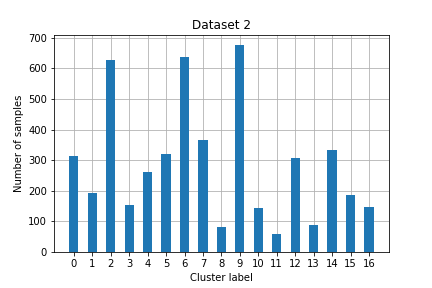
\includegraphics[width=.5\linewidth]{../../plots/gmm_hist_2}
			\caption{Distribution of samples across GMM clusters}
			\label{fig:gmm_hist}
		\end{minipage}%
	\end{figure}

	As the data is high-dimensional, parallel coordinates plots with a random subset of features along with the ground truth labels were used for visualization as shown in figure \ref{fig:kmeans_viz}. We can observe that samples belonging to a cluster occupy a small range along each feature. Some clusters are noisy and span larger ranges along some features. Some clusters (e.g. cluster 3 in dataset 1) correspond to specific ground truth labels while other clusters are noisy in this respect.
	
	\begin{figure}
		\centering
		\begin{minipage}{.5\textwidth}
			\centering
			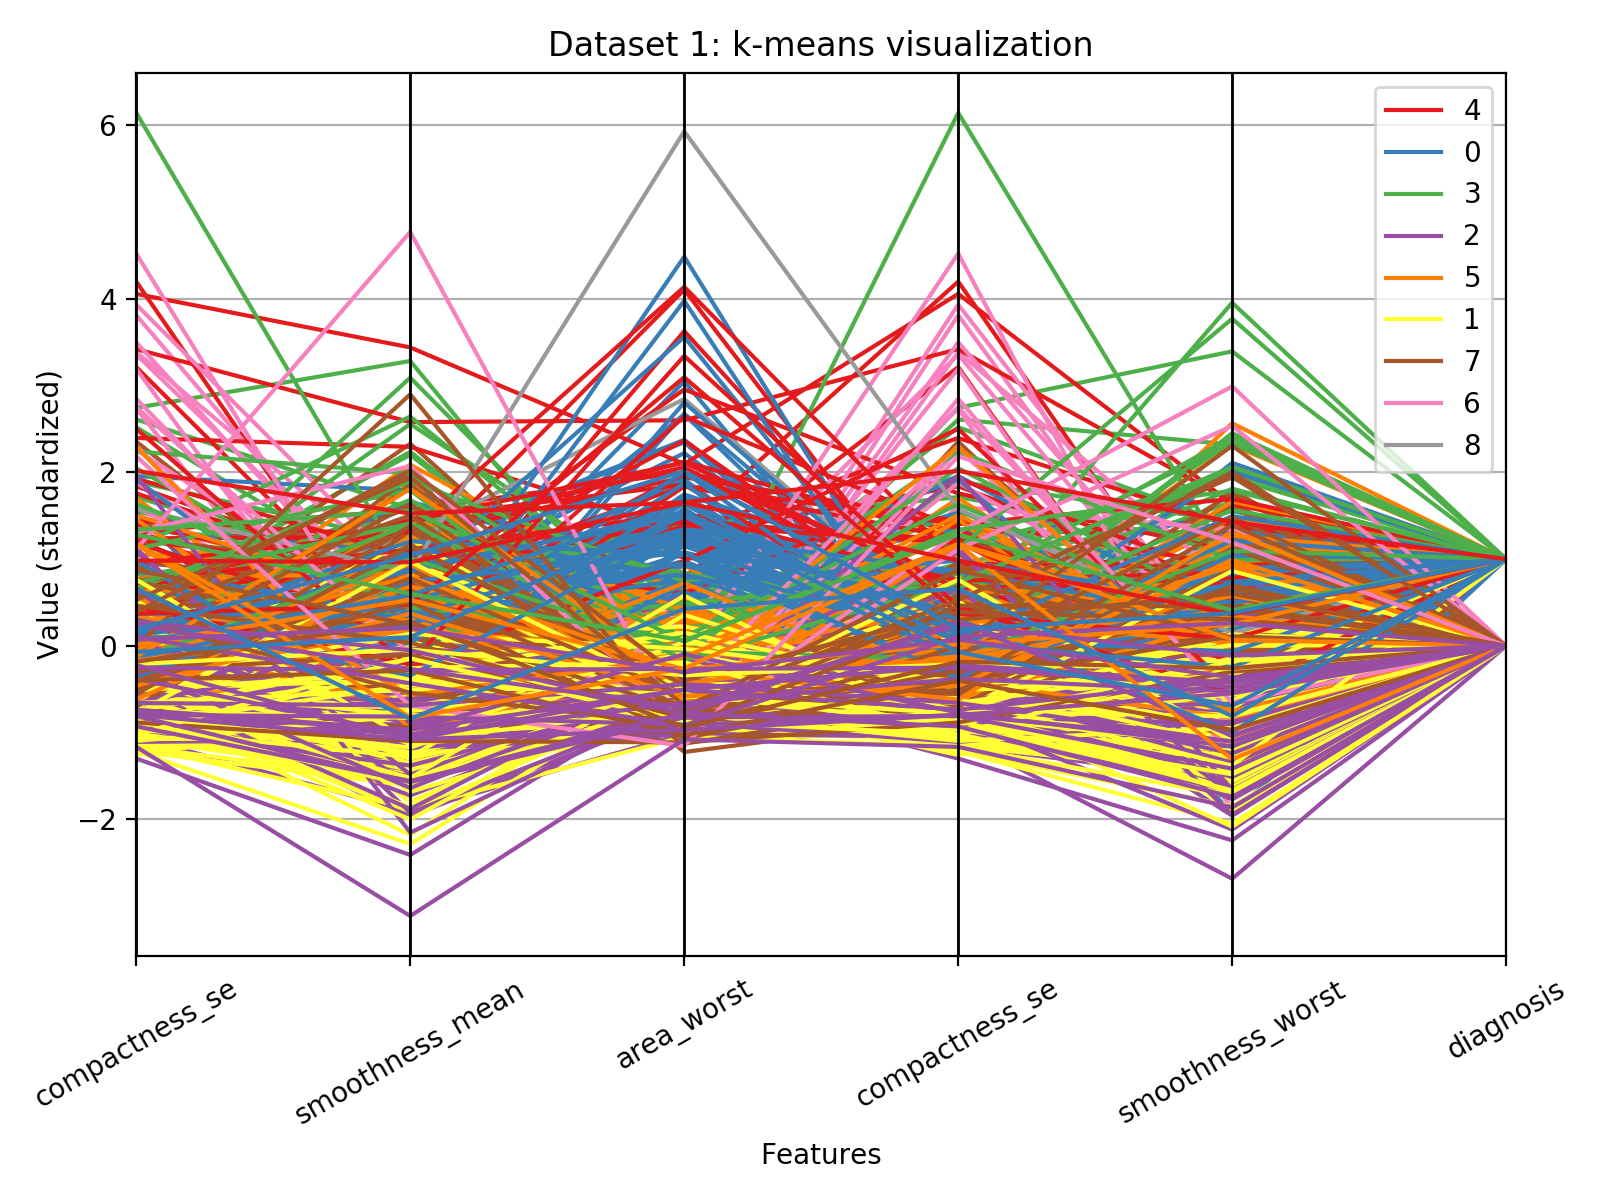
\includegraphics[width=\linewidth]{../../plots/kmeans_viz_1}
			%\caption{Loss curve for RHC}
		\end{minipage}%
		\begin{minipage}{.5\textwidth}
			\centering
			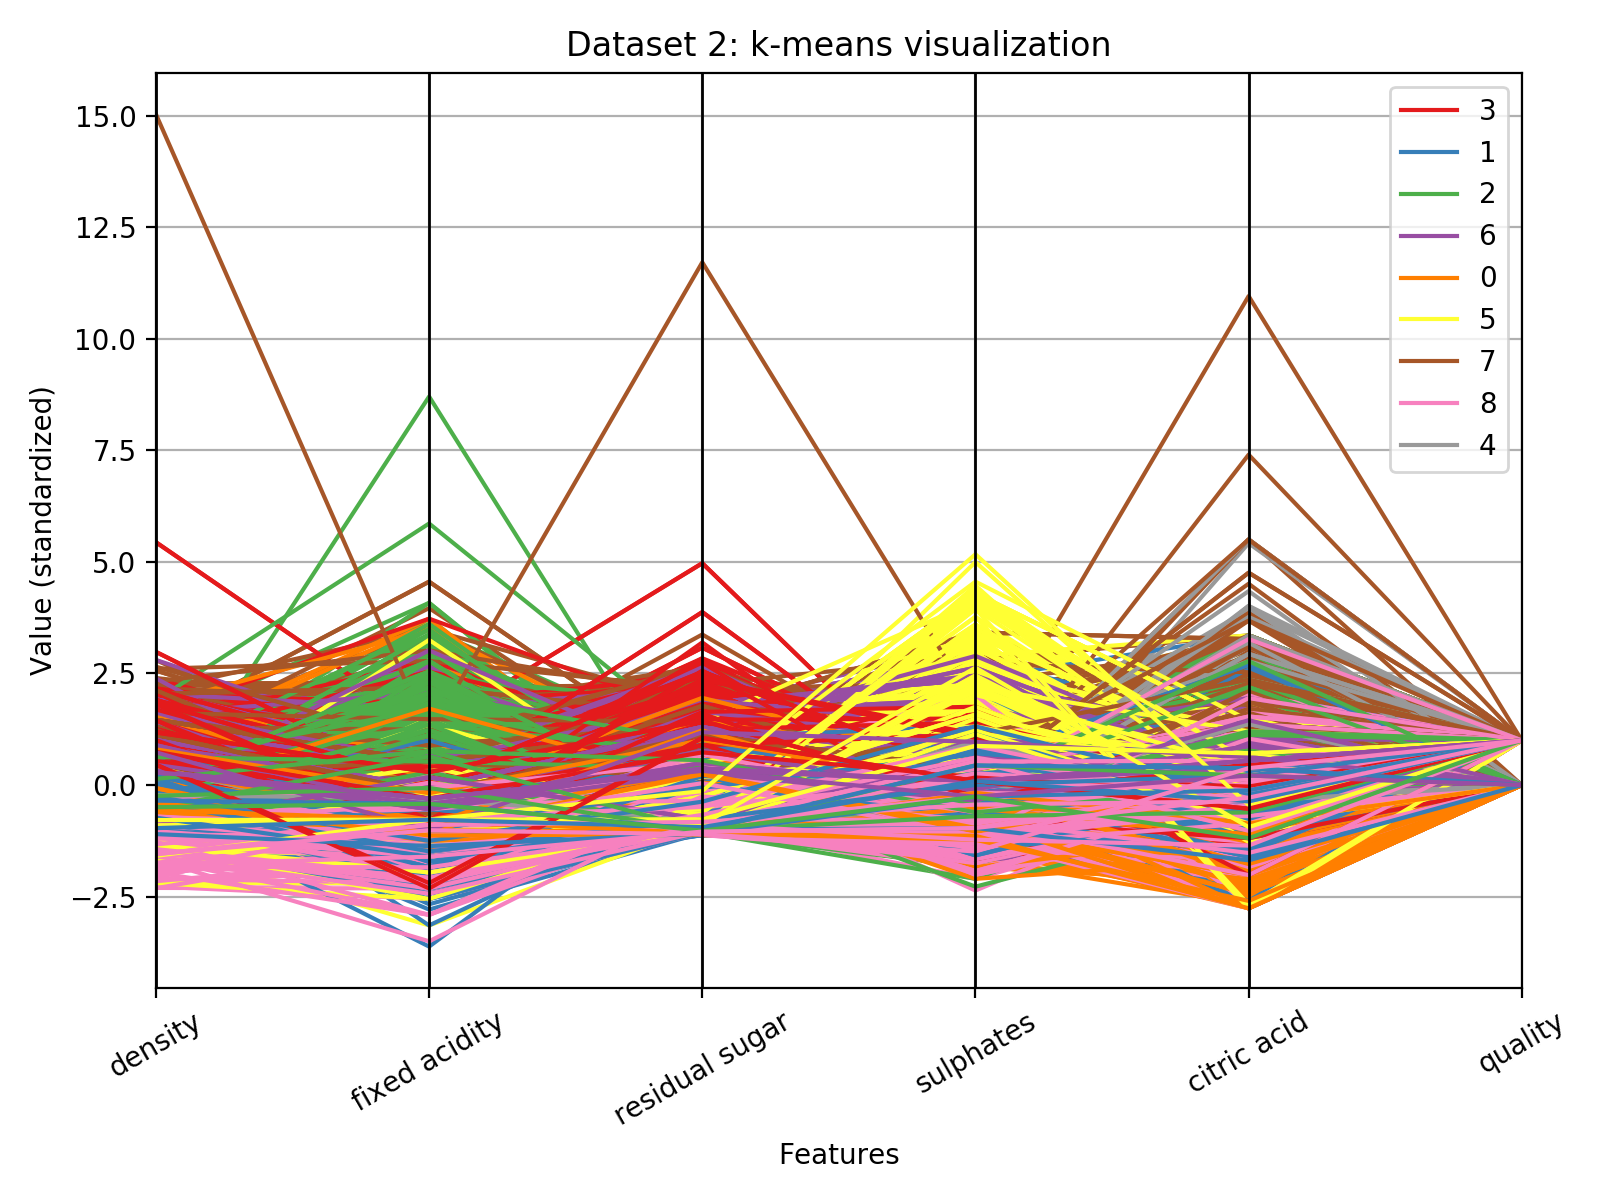
\includegraphics[width=\linewidth]{../../plots/kmeans_viz_2}
			%\caption{Loss for different runs of RHC}		
		\end{minipage}
		\caption{K-means visualization (without PCA)}
		\label{fig:kmeans_viz}
	\end{figure}
	
	Silhouette Coefficient score was used to evaluate clustering performance \cite{rousseeuwSilhouettesGraphicalAid1987}. It is a measure of how similar a sample is to its own cluster (cohesion) compared to other clusters (separation). It is defined for each sample and the mean Silhouette Coefficient score across samples was used as the evaluation metric. The score is bounded between -1 and 1. Scores close to 1 indicate that samples are far away from the neighboring clusters. A value near 0 indicates that the samples are on or very close to the decision boundary between neighboring clusters. A negative value indicates that some samples might have been assigned to the wrong cluster.
	
	The Silhouette Coefficient scores for the two datasets are reported in table \ref{tab:silhouette_bic1}. The scores are 0.15 and 0.13 which indicate that many samples are close to the decision boundary between neighboring clusters and the clusters aren't well-separated. The absence of a prominent elbow suggested that k-means may not be able to find good clusters and this observation reinforces the point. The mediocre clustering performance might be because of outliers in the data or convergence to a local optimum. The k-means++ initialization method and multiple initializations increase the probability of finding the global optimum but don't guarantee it. Another reason might be that the clusters in the data, if present, aren't spherical. K-means assumes spherical clusters and might be struggling to find the actual clusters due to this constraint.
	
	\begin{table}[]
		\centering
		\caption{Clustering performance evaluation}
		\label{tab:silhouette_bic1}
		\begin{tabular}{@{}ccccc@{}}
			\toprule
			\textbf{} & \multicolumn{2}{c}{\textbf{Dataset 1 (k = 9)}} & \multicolumn{2}{c}{\textbf{Dataset 2 (k = 9)}} \\ \midrule
			& \begin{tabular}[c]{@{}c@{}}K-means \\ silhouette score\end{tabular} & GMM BIC score & \begin{tabular}[c]{@{}c@{}}K-means \\ silhouette score\end{tabular} & GMM BIC score \\ \midrule
			Without PCA & 0.15 & 5869 & 0.13 & 109069 \\ \midrule
			With PCA & 0.19 & 12984 & 0.14 & 95844 \\ \bottomrule
		\end{tabular}
	\end{table}
	
	To assess how well the clusters line up with the ground truth labels, Adjusted Mutual Information (AMI) was used \cite{vinhInformationTheoreticMeasures2009}. AMI measures the agreement between two assignments, ignoring permutations. It is bounded between 0 and 1. Values close to 0 indicate two label assignments that are largely independent, while values close to 1 indicate significant agreement.
	
	The AMI scores for the two datasets are reported in table \ref{tab:ami1}. The scores of 0.24 and 0.04 indicate that the clusters line up with the labels somewhat well in case of dataset 1 but not for dataset 2. In general, for binary classification, clusters will line up with the labels when the data is separable with a series of hyperplanes because k-means operates on Euclidean distances in the feature space. In assignment 1, it was observed that linear classifiers worked well on dataset 1 with accuracies greater than 95\% whereas they did not perform so well on dataset 2 with accuracies around 75\%. The AMI scores are consistent with this observation.
	
	\begin{table}[]
		\centering
		\caption{AMI scores}
		\label{tab:ami1}
		\begin{tabular}{@{}ccccccc@{}}
			\toprule
			\textbf{Clustering method} & \multicolumn{3}{c}{\textbf{Dataset 1}} & \multicolumn{3}{c}{\textbf{Dataset 2}} \\ \midrule
			& \begin{tabular}[c]{@{}c@{}}k/number of \\ components\end{tabular} & \begin{tabular}[c]{@{}c@{}}Without \\ PCA\end{tabular} & \begin{tabular}[c]{@{}c@{}}With \\ PCA\end{tabular} & \begin{tabular}[c]{@{}c@{}}k/number of \\ components\end{tabular} & \begin{tabular}[c]{@{}c@{}}Without \\ PCA\end{tabular} & \begin{tabular}[c]{@{}c@{}}With \\ PCA\end{tabular} \\ \midrule
			K-means & 9 & 0.24 & 0.23 & 9 & 0.04 & 0.03 \\ \midrule
			GMM-EM & 5 & 0.24 & 0.29 & 17 & 0.03 & 0.03 \\ \bottomrule
		\end{tabular}
	\end{table}

	The cost function of k-means, i.e. inertia is biased towards spherical clusters. Moreover, it is not a normalized metric. Euclidean distances tend to become inflated in high-dimensional spaces and PCA may be used to alleviate this problem. This is explored in the next set of experiments. A kernel may be used to project the data to a different space where clusters may be well-formed. A GMM may be used in cases where k-means fails since it is a soft clustering algorithm and is more flexible.
	
	\begin{figure}
		\centering
		\begin{minipage}{.5\textwidth}
			\centering
			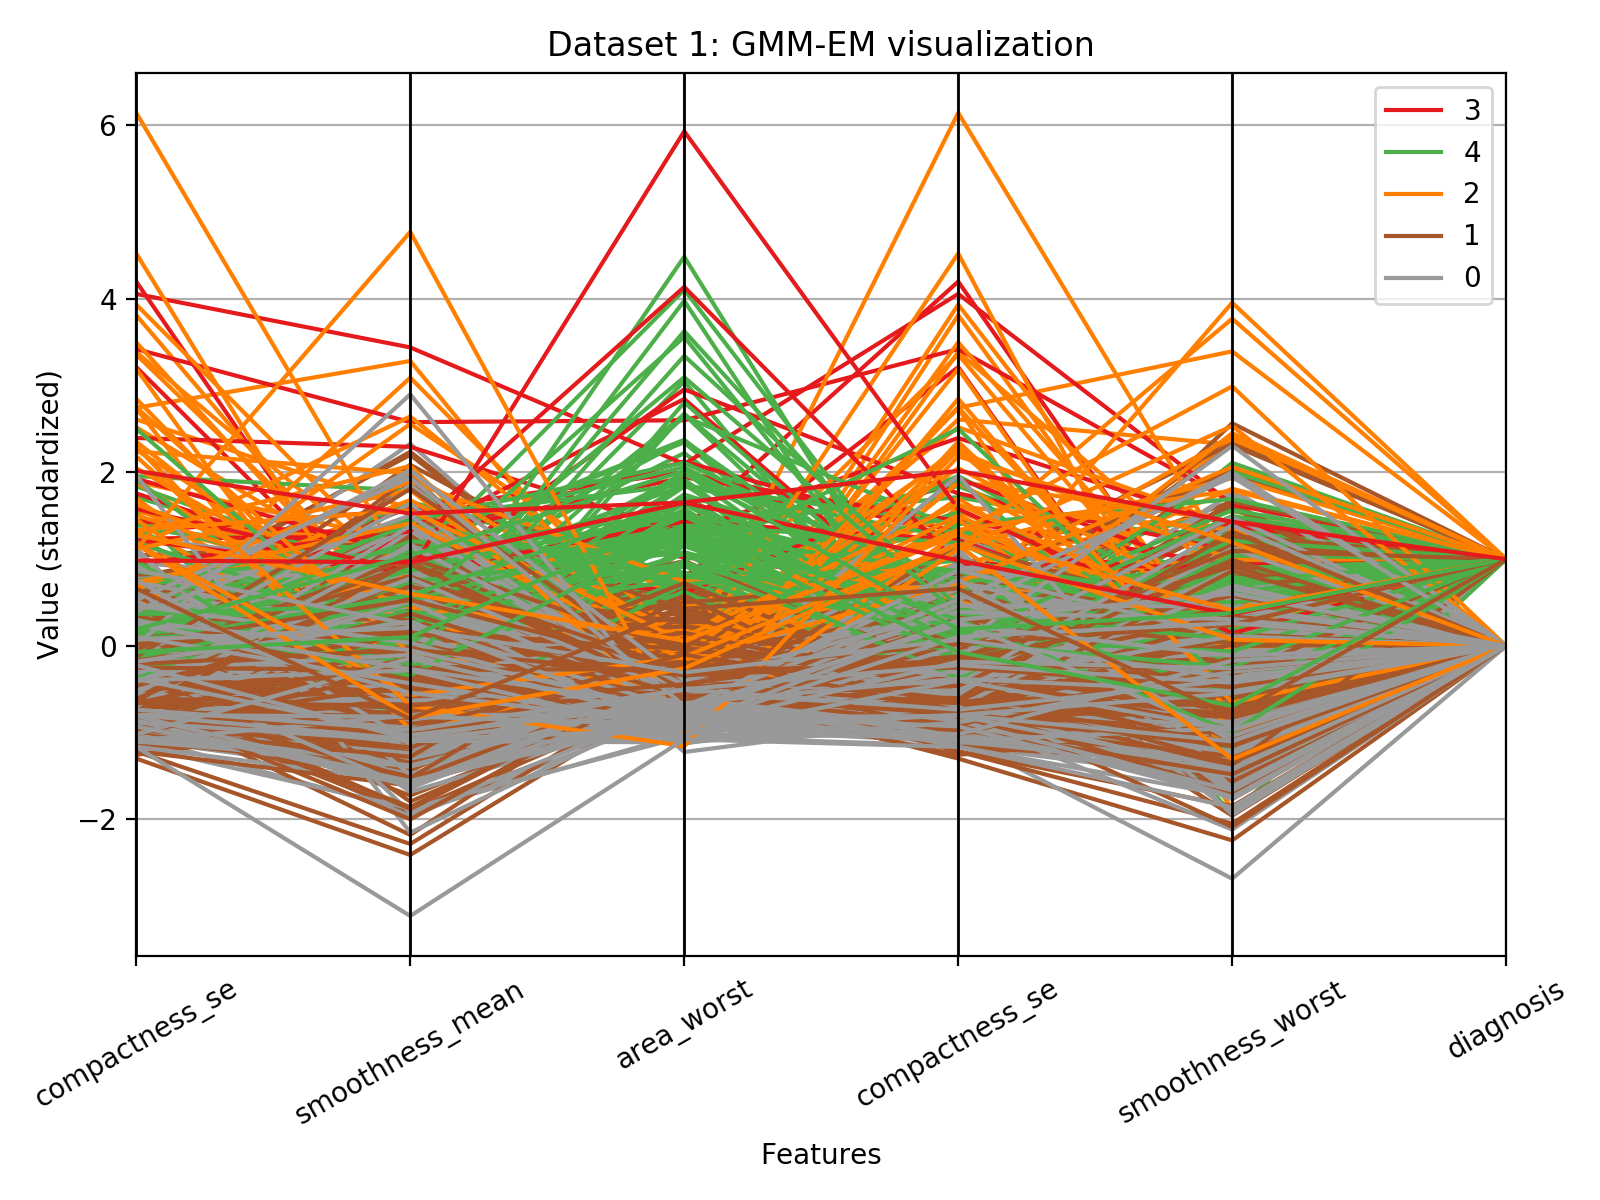
\includegraphics[width=\linewidth]{../../plots/gmm_viz_1}
			%\caption{Loss curve for RHC}
		\end{minipage}%
		\begin{minipage}{.5\textwidth}
			\centering
			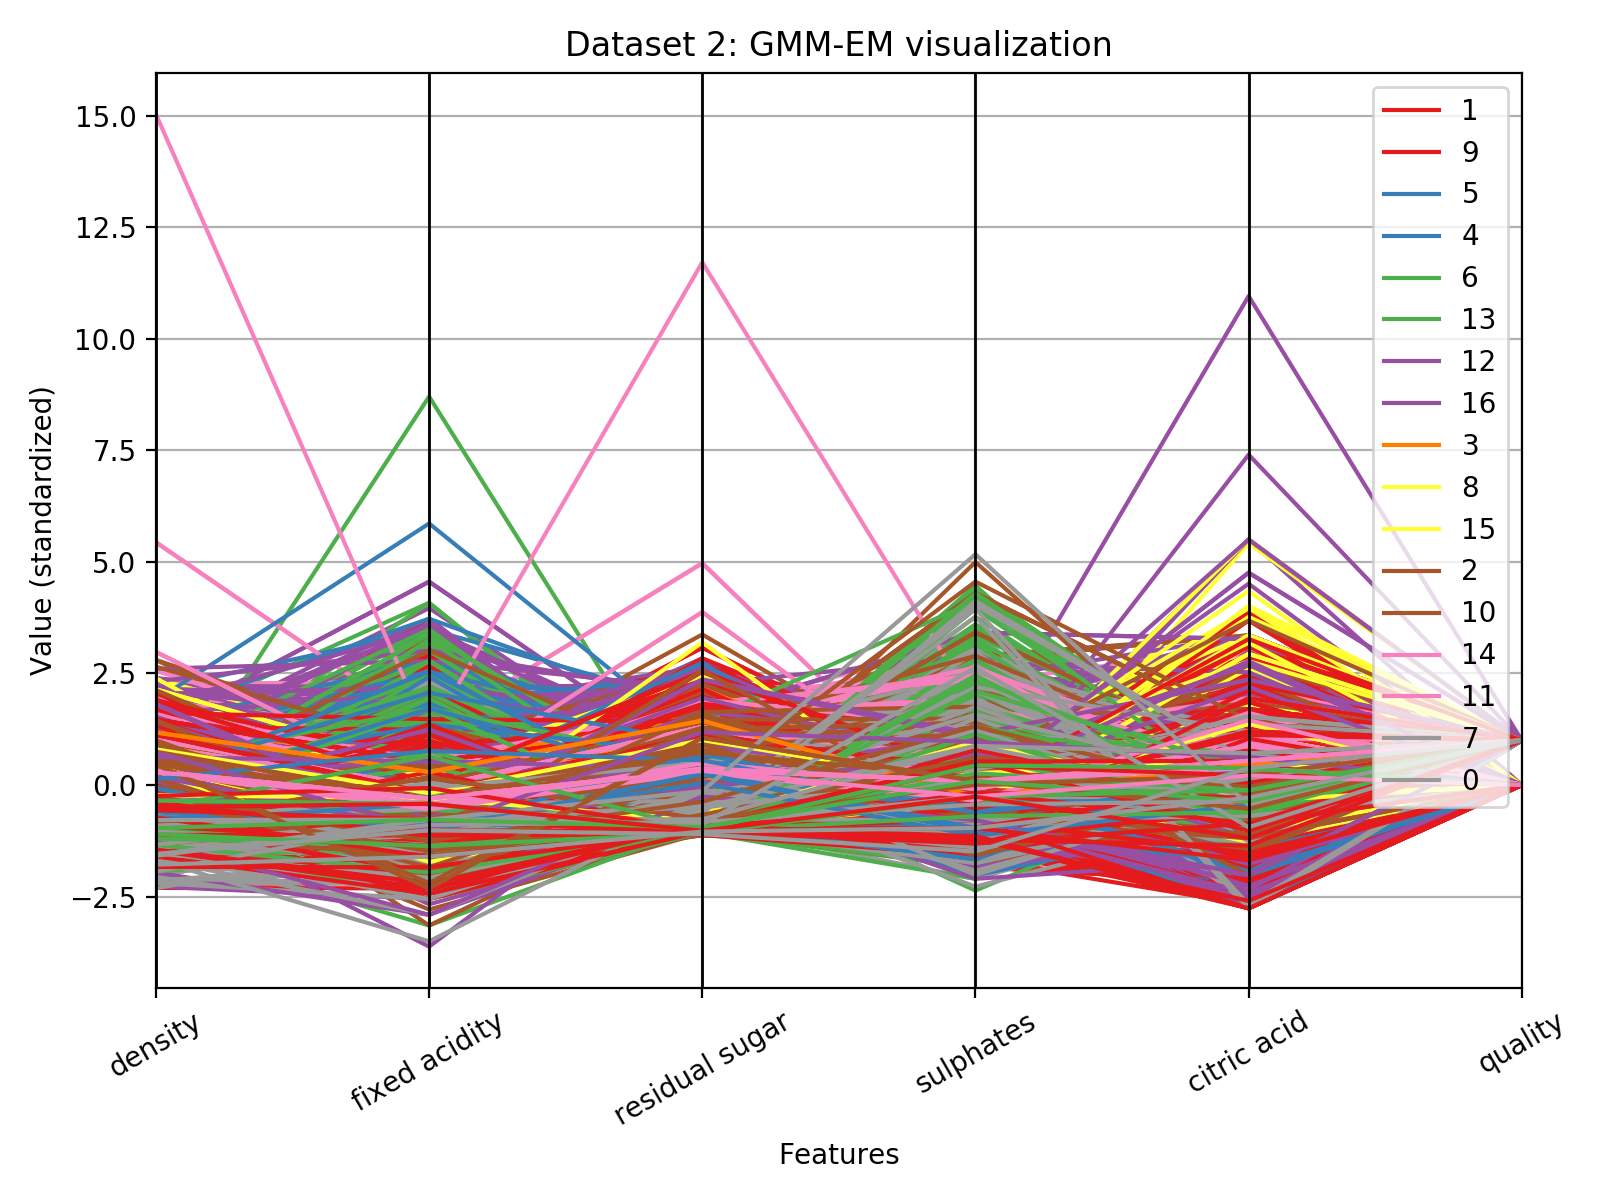
\includegraphics[width=\linewidth]{../../plots/gmm_viz_2}
			%\caption{Loss for different runs of RHC}		
		\end{minipage}
		\caption{GMM visualization (without PCA)}
		\label{fig:gmm_viz}
	\end{figure}	

	\subsubsection{GMM-EM}
	\begin{figure}
		\centering
		\begin{minipage}{.5\textwidth}
			\centering
			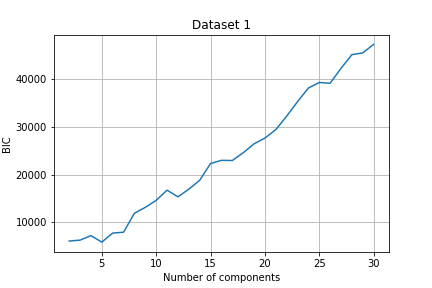
\includegraphics[width=\linewidth]{../../plots/gmm_bic_1}
			%\caption{Loss curve for RHC}
		\end{minipage}%
		\begin{minipage}{.5\textwidth}
			\centering
			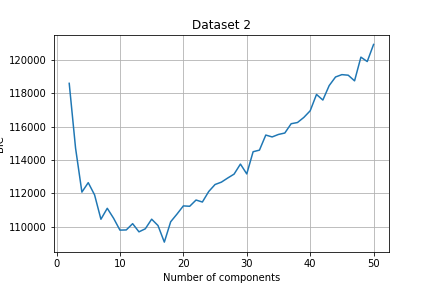
\includegraphics[width=\linewidth]{../../plots/gmm_bic_2}
			%\caption{Loss for different runs of RHC}		
		\end{minipage}
		\caption{BIC for different number of GMM components}
		\label{fig:gmm_bic}
	\end{figure}

	The Bayesian Information Criterion (BIC) was used to select the number of components in the GMMs. It tries to maximize log-likelihood of data while penalizing the number of parameters in the model to prevent overfitting. In theory, it recovers the true number of components in the asymptotic regime where the data contains an infinite number of samples generated iid from a Gaussian mixture. Lower BIC values are better.
	
	Figure \ref{fig:gmm_bic} shows BIC for varying number of GMM components. The number of components was chosen based on the location of minima which was 5 and 17 for datasets 1 and 2 respectively. Figure \ref{fig:gmm_hist} shows the distribution of data across clusters. Again it is uneven with some clusters having much more samples than others. Parallel coordinates plots for the two datasets with random subsets of features are shown in figure \ref{fig:gmm_viz}. The Gaussian weights are plotted in figure \ref{fig:gmm_wts_viz}. The maximum posterior probabilities of a sample belonging to a cluster are plotted in figure \ref{fig:gmm_probs_viz}. The clustering for dataset 1 is quite hard, similar to k-means while it is softer for dataset 2.

	\begin{figure}
		\centering
		\begin{minipage}{.48\textwidth}
			\centering
			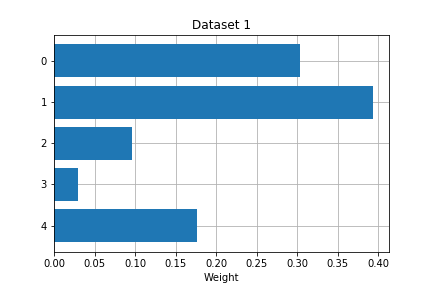
\includegraphics[width=.5\linewidth]{../../plots/gmm_wts_1}%
			\centering
			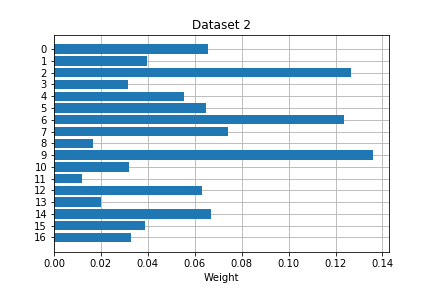
\includegraphics[width=.5\linewidth]{../../plots/gmm_wts_2}
			\caption{Visualization of GMM weights (without PCA)}
			\label{fig:gmm_wts_viz}
		\end{minipage}%
		\hfill
		\begin{minipage}{.48\textwidth}
			\centering
			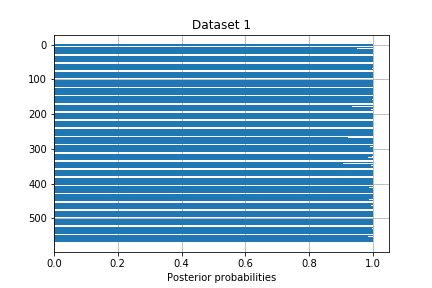
\includegraphics[width=.5\linewidth]{../../plots/gmm_probs_1}%
			\centering
			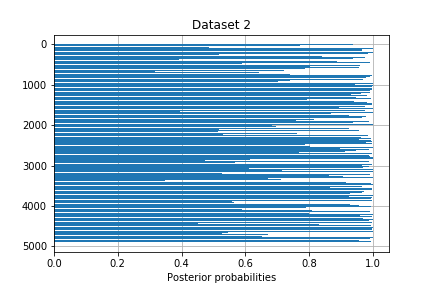
\includegraphics[width=.5\linewidth]{../../plots/gmm_probs_2}
			\caption{GMM maximum posterior probabilities (without PCA)}
			\label{fig:gmm_probs_viz}%
		\end{minipage}
	\end{figure}
	
	Silhouette Coefficient scores cannot be used to evaluate the performance of GMMs because they work well only on spherical clusters and GMMs do not necessarily produce spherical clusters. Instead, we will use BIC introduced previously. The BIC scores for the two datasets are reported in table \ref{tab:silhouette_bic1}. Note that the BIC of one dataset cannot be compared to that of the other. This is because they have different number of examples and components and BIC is increases with an increase in any of them.
	
	Similar to k-means, AMI was used to assess how well the clusters line up with the ground truth labels. The AMI scores are reported in table \ref{tab:ami1}. The scores are 0.24 and 0.03 respectively which are very close to the scores obtained with k-means. The clusters line up somewhat well in case of dataset 1 but not for dataset 2. As observed in case of k-means, the clusters line up well with the labels for datasets which are separable with a series of hyperplanes. As found in assignment 1, linear classifiers work well on dataset 1 but not on dataset 2. The AMI scores agree with this observation.
	
	\subsection{Clustering with dimensionality reduction}
	In this set of experiments, PCA was first applied to the datasets to reduce their dimensionality and then clustering was performed using k-means and GMM-EM. The same number of clusters/components as in the previous section was used and the results before and after PCA are compared.
	
	\subsubsection{PCA}
	The proportion of total variance in the data explained by each component which is also the corresponding eigenvalue of the covariance matrix is plotted in figure \ref{fig:pca_var} and the cumulative variance is plotted in figure \ref{fig:pca_cum_var}. Note how most of the variance is explained by the first few components. A good rule of thumb to select the number of components is to do it in a way such that the chosen components account for over 85\% of the variance. Thus, the number of components for the two datasets are 6 and 7 respectively. The reconstruction errors measured by the mean-squared error between the original data and the data produced by applying the inverse transform on the reduced data are 0.11 and 0.12 respectively.
	
	\begin{figure}
		\centering
		\begin{minipage}{.5\textwidth}
			\centering
			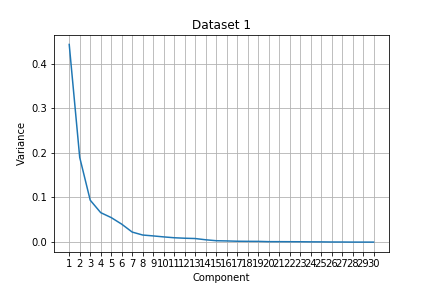
\includegraphics[width=.5\linewidth]{../../plots/pca_var_1}%
			\centering
			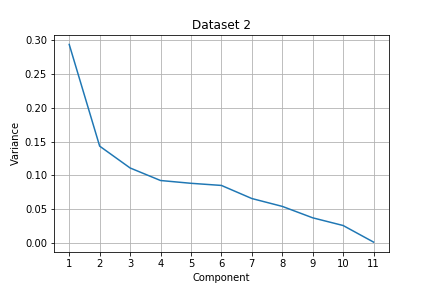
\includegraphics[width=.5\linewidth]{../../plots/pca_var_2}
			\caption{Variance for different components}
			\label{fig:pca_var}
		\end{minipage}%
		\begin{minipage}{.5\textwidth}
			\centering
			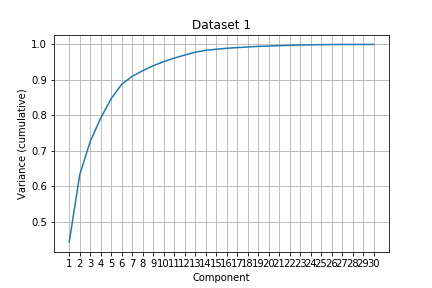
\includegraphics[width=.5\linewidth]{../../plots/pca_var_cum_1}%
			\centering
			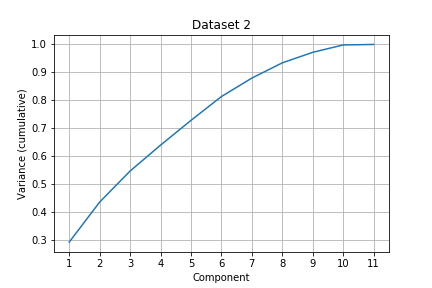
\includegraphics[width=.5\linewidth]{../../plots/pca_var_cum_2}
			\caption{Cumulative variance}
			\label{fig:pca_cum_var}
		\end{minipage}
	\end{figure}
	
	\subsubsection{K-means}
	The distribution of samples across k-means clusters is plotted in figure \ref{fig:pca_kmeans_hist} and parallel coordinates plots are shown in figure \ref{fig:pca_kmeans_viz}. We can observe that the clusters obtained after PCA are different. This is because the data is projected to a different, lower dimensional space. K-means produces clusters according to the spatial distribution of data and clustering in different spaces will result in different clusters.
	
	\begin{figure}
		\centering
		\begin{minipage}{.48\textwidth}
			\centering
			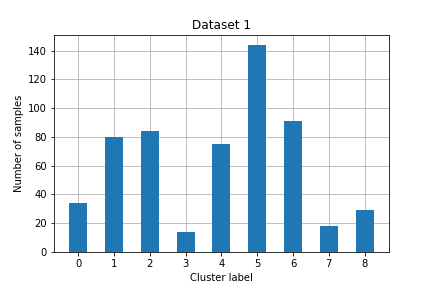
\includegraphics[width=.5\linewidth]{../../plots/pca_kmeans_hist_1}%
			\centering
			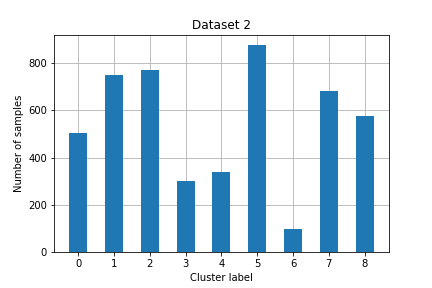
\includegraphics[width=.5\linewidth]{../../plots/pca_kmeans_hist_2}
			\caption{Distribution of samples across k-means clusters (after PCA)}
			\label{fig:pca_kmeans_hist}
		\end{minipage}%
		\hfill
		\begin{minipage}{.48\textwidth}
			\centering
			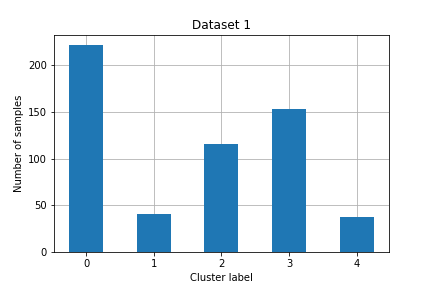
\includegraphics[width=.5\linewidth]{../../plots/pca_gmm_hist_1}%
			\centering
			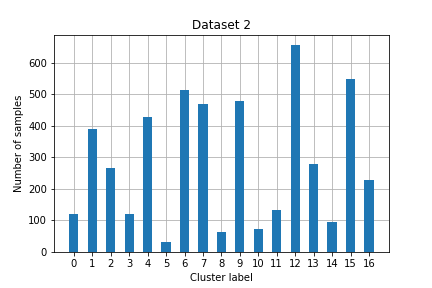
\includegraphics[width=.5\linewidth]{../../plots/pca_gmm_hist_2}
			\caption{Distribution of samples across GMM clusters (after PCA)}
			\label{fig:pca_gmm_hist}
		\end{minipage}%
	\end{figure}

	\begin{figure}
		\centering
		\begin{minipage}{.5\textwidth}
			\centering
			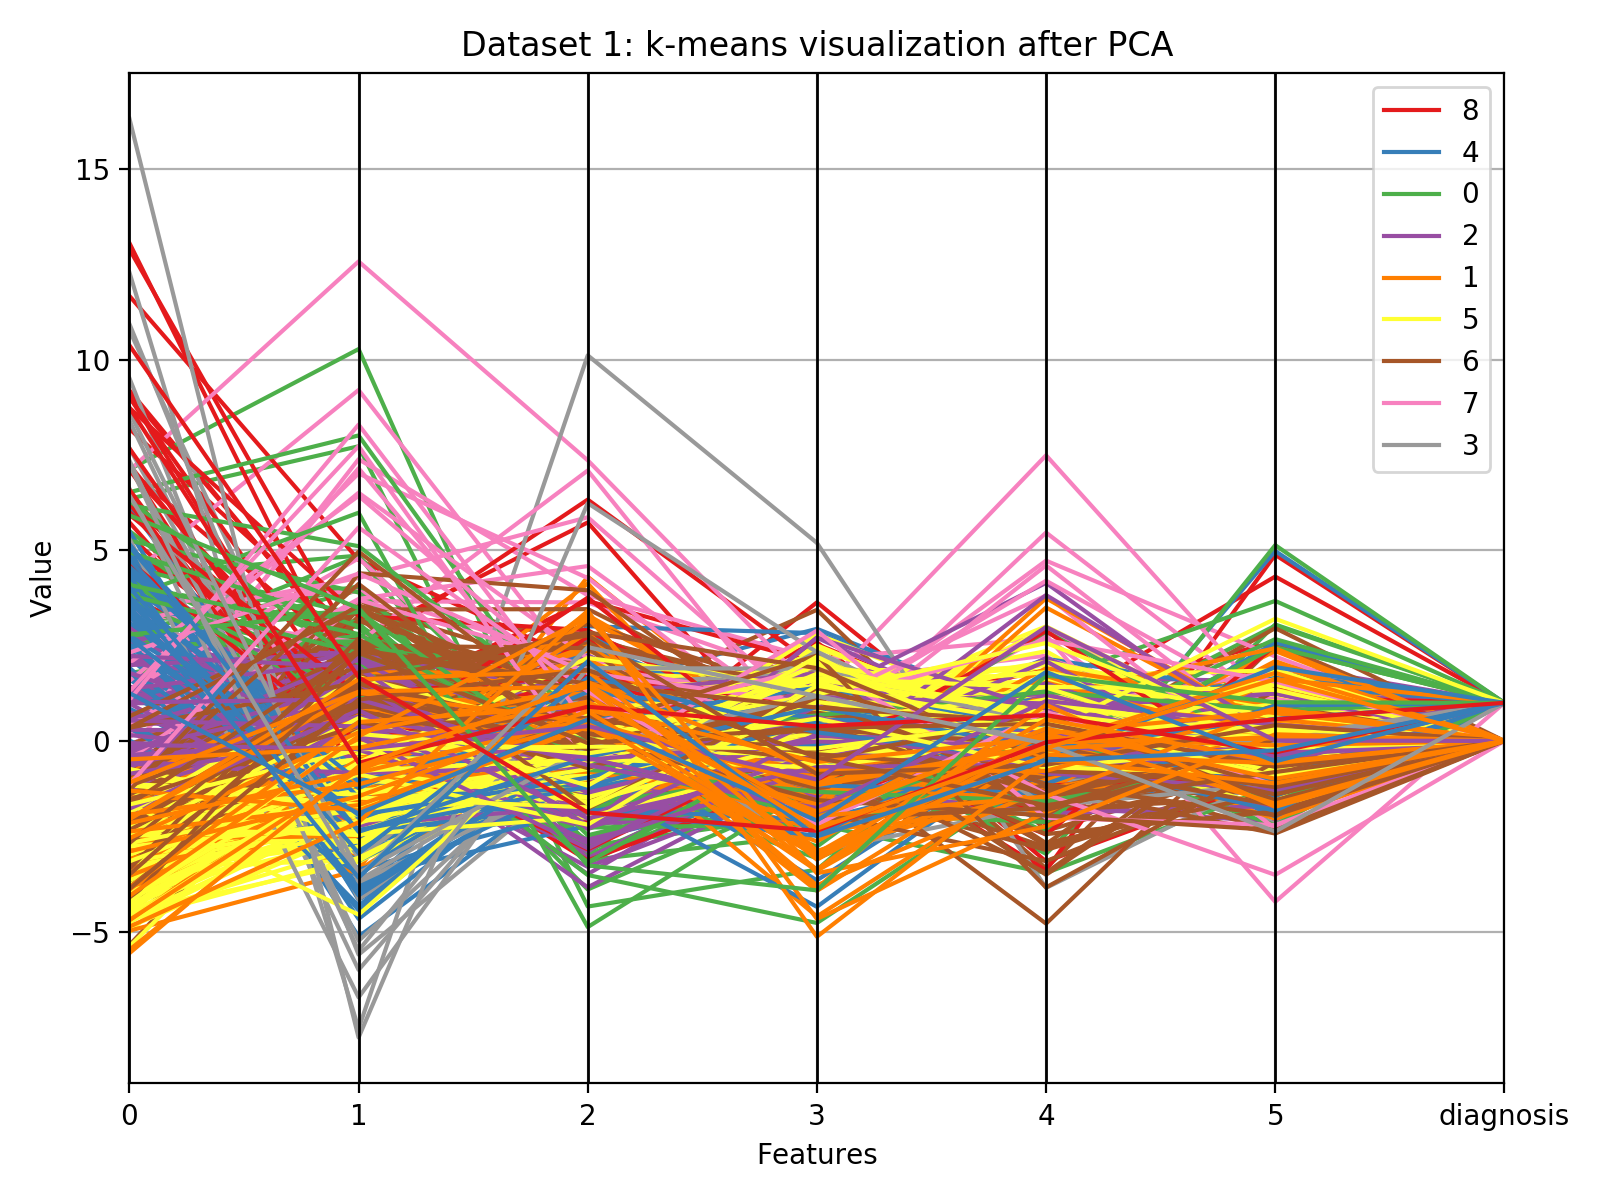
\includegraphics[width=\linewidth]{../../plots/pca_kmeans_viz_1}
			%\caption{Loss curve for RHC}
		\end{minipage}%
		\begin{minipage}{.5\textwidth}
			\centering
			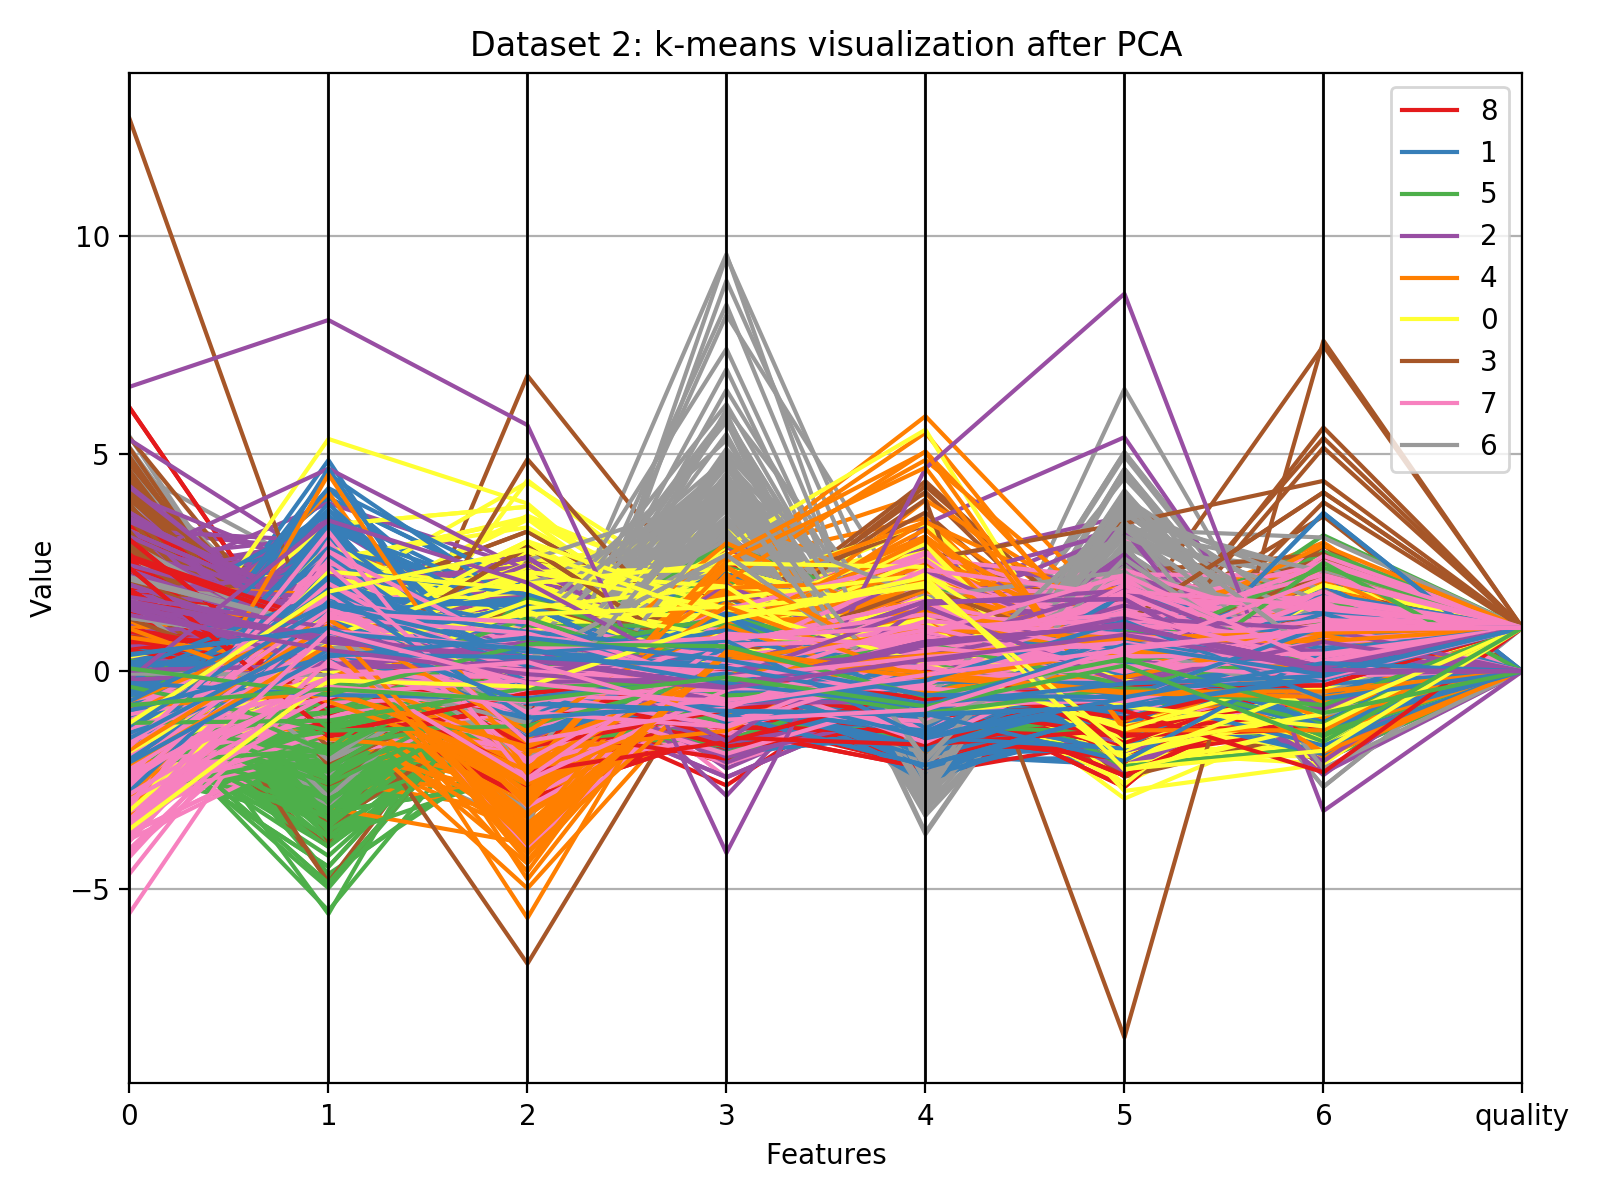
\includegraphics[width=\linewidth]{../../plots/pca_kmeans_viz_2}
			%\caption{Loss for different runs of RHC}		
		\end{minipage}
		\caption{K-means visualization (after PCA)}
		\label{fig:pca_kmeans_viz}
	\end{figure}

	The silhouette and AMI scores after PCA are reported in tables \ref{tab:silhouette_bic1} and \ref{tab:ami1} respectively. The silhouette scores for both datasets have increased after applying PCA which means that the quality of the clusters has improved after dimensionality reduction. This might be because noisy features might have been removed after PCA as k-means is sensitive to outliers. The AMI scores have slightly decreased after PCA. This is possibly because the separability of the data using hyperplanes has decreased.
	
	\subsubsection{GMM-EM}
	The distribution of GMM clusters is plotted in \ref{fig:pca_gmm_hist} and parallel coordinates plots are shown in figure \ref{fig:pca_gmm_viz}. The Gaussian weights are plotted in figure \ref{fig:pca_gmm_wts_viz}. Again, the clusters obtained after PCA are different because the data is in a lower-dimensional space and GMM clustering depends on spatial distribution of data. The maximum posterior probabilities are plotted in figure \ref{fig:pca_gmm_probs_viz}. Notice how the clustering after applying PCA is much softer.
	
	\begin{figure}
		\centering
		\begin{minipage}{.5\textwidth}
			\centering
			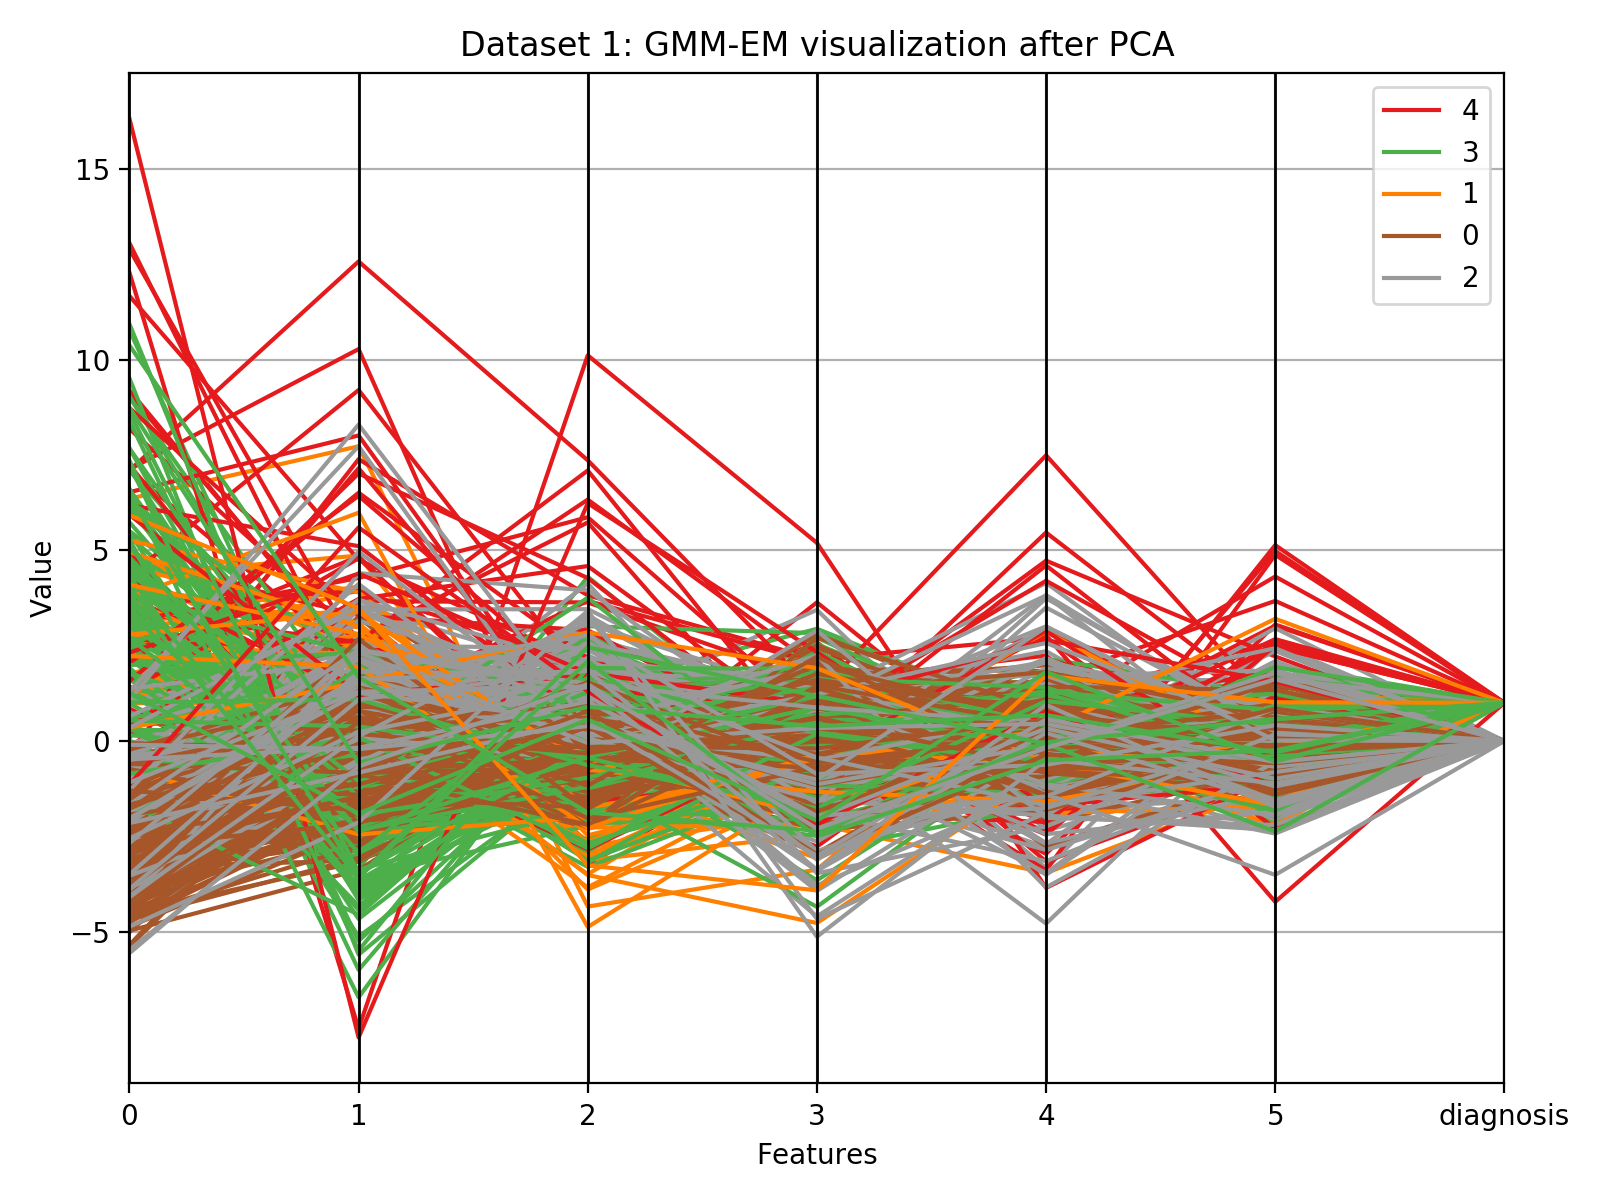
\includegraphics[width=\linewidth]{../../plots/pca_gmm_comp_viz_1}
			%\caption{Loss curve for RHC}
		\end{minipage}%
		\begin{minipage}{.5\textwidth}
			\centering
			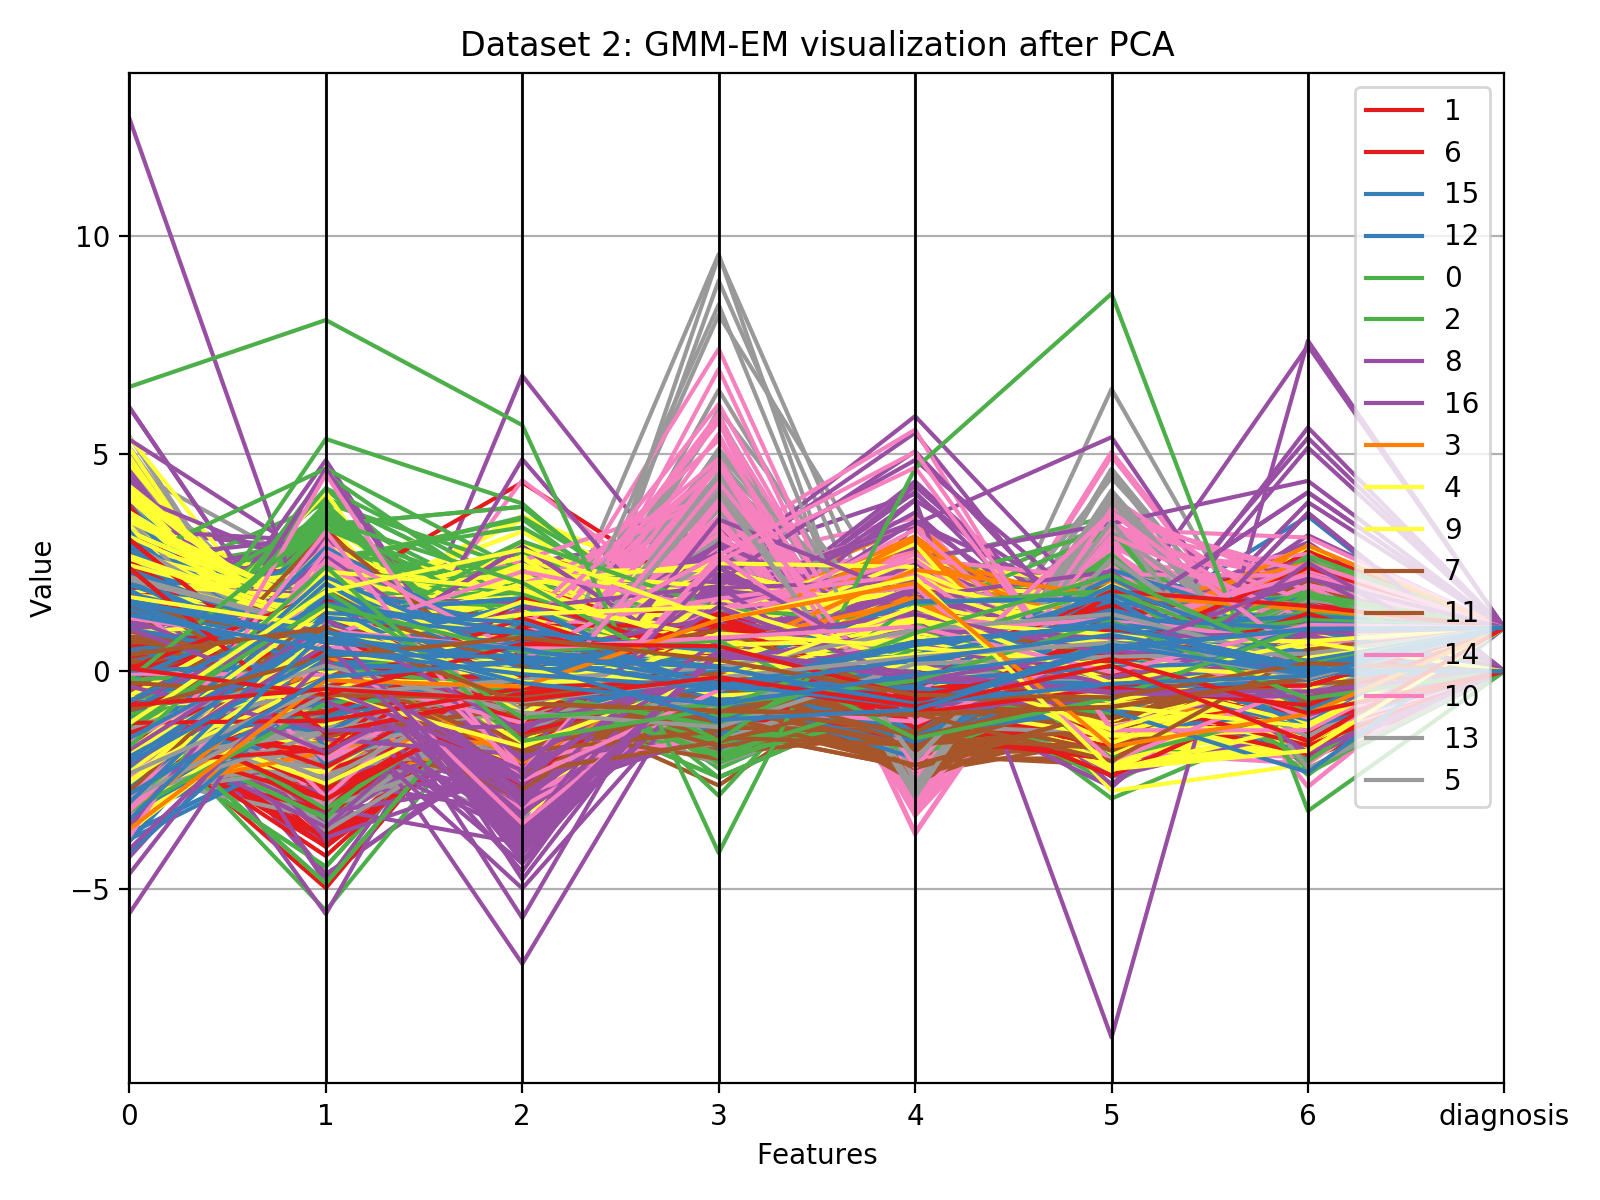
\includegraphics[width=\linewidth]{../../plots/pca_gmm_comp_viz_2}
			%\caption{Loss for different runs of RHC}		
		\end{minipage}
		\caption{GMM visualization (after PCA)}
		\label{fig:pca_gmm_viz}
	\end{figure}

	\begin{figure}
		\centering
		\begin{minipage}{.48\textwidth}
			\centering
			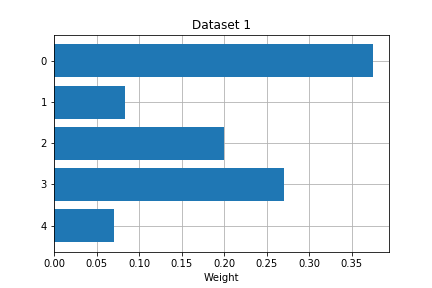
\includegraphics[width=.5\linewidth]{../../plots/pca_gmm_wts_1}%
			\centering
			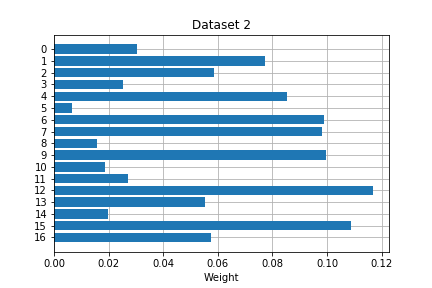
\includegraphics[width=.5\linewidth]{../../plots/pca_gmm_wts_2}
			\caption{Visualization of GMM weights (with PCA)}
			\label{fig:pca_gmm_wts_viz}
		\end{minipage}%
		\hfill
		\begin{minipage}{.48\textwidth}
			\centering
			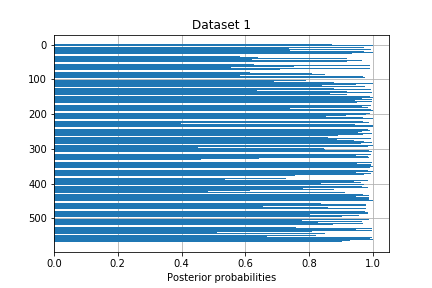
\includegraphics[width=.5\linewidth]{../../plots/pca_gmm_probs_1}%
			\centering
			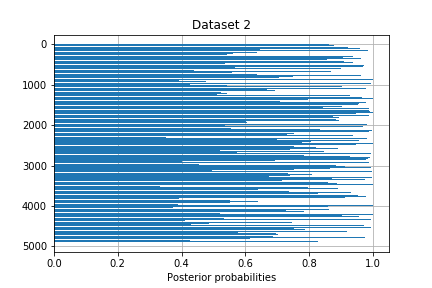
\includegraphics[width=.5\linewidth]{../../plots/pca_gmm_probs_2}
			\caption{GMM maximum posterior probabilities (with PCA)}
			\label{fig:pca_gmm_probs_viz}
		\end{minipage}%
	\end{figure}

	The BIC and AMI scores after PCA are reported in tables \ref{tab:silhouette_bic1} and \ref{tab:ami1} respectively. The BIC score for dataset 1 has increased while that for dataset 2 has decreased. This means that the quality of GMM clusters has got worse for dataset 1 and better for dataset 2. The AMI score for dataset 1 has improved while that of dataset has stayed the same. Again, this might be because the separability of the data using hyperplanes has decreased.
	
	\subsection{Neural network classification after dimensionality reduction}
	This set of experiments was performed on dataset 1. First, PCA was applied on the training set and the neural network used in assignment 1 was trained on the newly projected data. Next, the two clustering algorithms were used as dimensionality reduction algorithms and the projected data was again used to train the neural network. For k-means, the distances of the samples to the cluster centers were used as features. For GMM, the probabilities of the samples belonging to each cluster were used as features. Note that the dimensionality reduction projection was learned from the training set only.
	
	For each algorithm, a grid search with five-fold cross-validation was performed to find the optimal hyperparameters, viz. learning rate and regularization parameter. The test accuracies and training times are reported in table \ref{tab:nn}. The training time for all algorithms is more than training without any dimensionality reduction. This is because all dimensionality reduction algorithms used here are lossy. Some discriminative features in the original data might have been lost due to which the network took more time to converge. However, inspite of information loss, a network with PCA performs as good as one without dimensionality reduction, followed closely by k-means. This might be because the projected data still has enough discriminative features which the network is able to find. This might not be the case with GMM-EM due to which the accuracy drops in this case. Among the dimensionality reduction algorithms, PCA performs the best. This is because among all dimensionality reduction algorithms, PCA gives the best low-rank approximation of the data. Thus, information loss is minimal and the neural network still works well.
	
	\begin{table}[]
		\centering
		\caption{Performance metrics for different dimensionality reduction algorithms}
		\label{tab:nn}
		\begin{tabular}{@{}lll@{}}
			\toprule
			\textbf{Dimensionality reduction algorithm} & \textbf{Training time (seconds)} & \textbf{Test accuracy (\%)} \\ \midrule
			None & 0.155 & 97.81 \\ \midrule
			PCA & 0.323 & 97.81 \\ \midrule
			K-means & 0.39 & 96.05 \\ \midrule
			GMM-EM & 1.241 & 90.35 \\ \bottomrule
		\end{tabular}
	\end{table}

	\bibliographystyle{unsrt}
	\bibliography{cs7641-a3}
	
\end{document}